% Please make sure you insert your
% data according to the instructions in PoSauthmanual.pdf
\documentclass{PoS}

\title{Diffractive PDF determination from HERA inclusive and jet data at NNLO QCD}

\ShortTitle{Diffractive PDF determination from HERA inclusive and di-jet data at NNLO QCD}

\author{\speaker{Radek \v{Z}leb\v{c}\'{i}k}\\ on behalf of the \textup{\textbf{H1 Collaboration}} \\
        DESY\\
        E-mail: \email{radek.zlebcik@desy.de}}

%\author{Another Author\\
%        Affiliation\\
%        E-mail: \email{...}}


%\usepackage[utf8]{inputenc}
\usepackage{xspace}
\usepackage{amsmath}
\usepackage{amssymb}
\usepackage{paralist}



\newcommand{\IP}{I\!\!P}
\newcommand{\IR}{I\!\!R}
\newcommand{\xpom}{x_{\IP}}

\newcommand{\GeV}{\ensuremath{\mathrm{GeV}}\xspace}
\newcommand{\GeVsq}{\ensuremath{\mathrm{GeV}^2}\xspace}

%\newcommand{\includegraphicss} 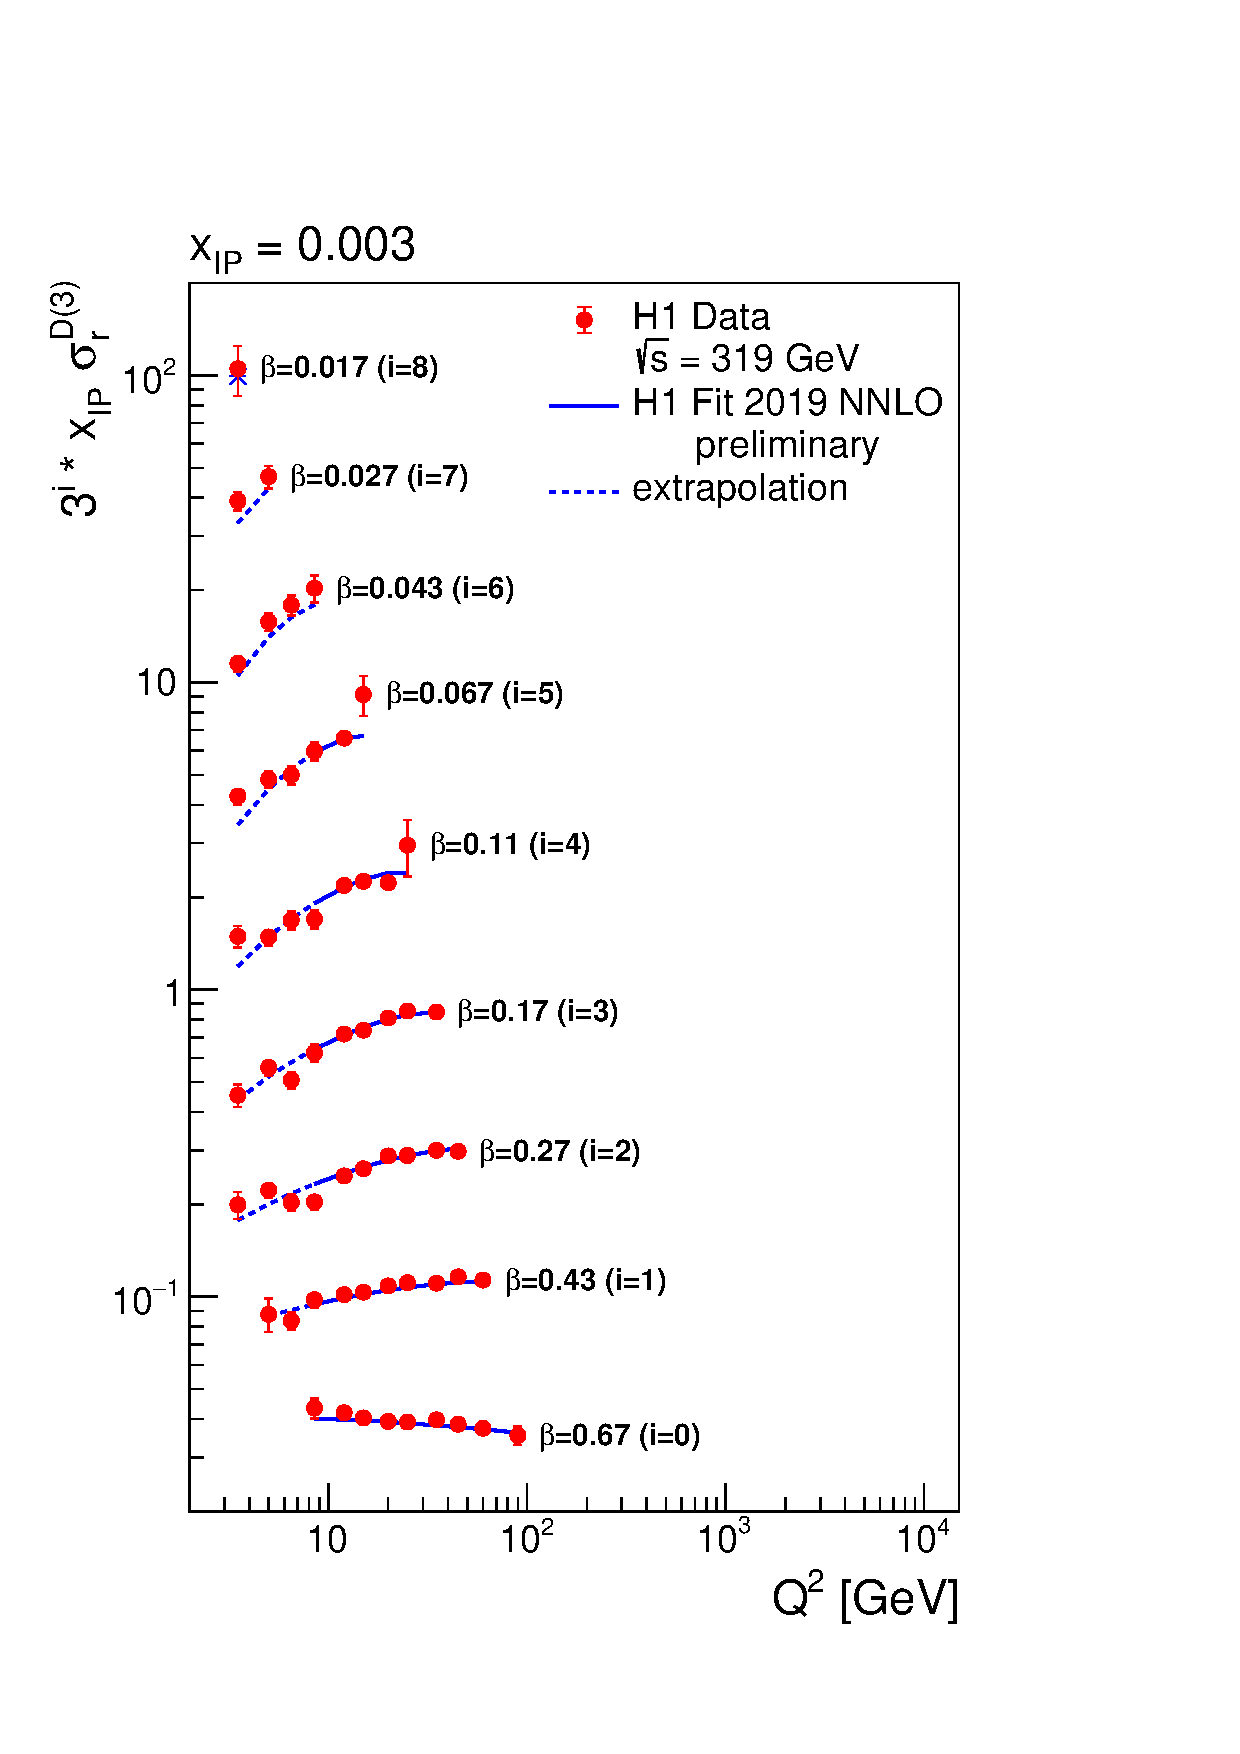
\includegraphics[width=.9\textwidth]{{{plots/H1prelim-19-013.fig10}}}

%\newcommand{\includegraphicss}[2][]{\fbox{\includegraphics[#1]{#2}}}
\newcommand{\includegraphicss}[2][]{\includegraphics[#1]{#2}}
%            Mandatory arg: #2; Optional arg: #1.}


\makeatletter
\newcommand*{\rom}[1]{\expandafter\@slowromancap\romannumeral #1@}
\makeatother


% the six measurements
\newcommand{\HERAI} {\protect\scalebox{0.8}{(HERA~\rom{1})}}
\newcommand{\HERAII} {\protect\scalebox{0.8}{(HERA~\rom{2})}}
\newcommand{\LowEP} {\protect\scalebox{0.8}{($300\,\GeV$)}}
\newcommand{\HLRG}  {H1~LRG~\HERAII\xspace}
\newcommand{\HVFPS} {H1~VFPS~\HERAII\xspace}
\newcommand{\HFPS}  {H1~FPS~\HERAII\xspace}
\newcommand{\HLRGI} {H1~LRG~\HERAI\xspace}
\newcommand{\ZLRG}  {ZEUS~LRG~\HERAI\xspace}
\newcommand{\HLRGEp}{H1~LRG~\LowEP\xspace}



\abstract{A new fit of diffractive parton distribution functions (DPDFs) to the HERA inclusive and di-jet data in diffractive deep-inelastic scattering (DDIS) at next-to-next-to-leading order accuracy (NNLO) is presented. The inclusion of the most comprehensive dijet cross section data, together with their NNLO predictions, provide enhanced constraints to the gluon component of the DPDF, which is of particular importance for diffractive PDFs. Compared to previous HERA fits, the presented fit includes the high-precision HERA~II data of the H1 collaboration, which corresponds to a 40-fold increase in luminosity for inclusive data and six-fold increase for di-jet data. In addition to the inclusive DDIS data sample at the nominal centre-of-mass energy $\sqrt{s} = 319\,\GeV$, H1 data at $252$~GeV and $225$~GeV are included. The extracted DPDFs are compared to previous DPDF fits and are used to predict cross sections for a large number of available measurements and differential observables.}

\FullConference{XXVII International Workshop on Deep-Inelastic Scattering and Related Subjects - DIS2019\\
		8-12 April, 2019\\
		Torino, Italy}


\begin{document}

\section{Introduction}

Diffractive processes, $ep \to  eXY$, where the systems $X$ and $Y$ are separated in rapidity, have been studied extensively at the electron-proton collider HERA.
The forward system $Y$ usually consists of the leading proton but can also contain its low mass dissociation.
Between the systems $X$ and $Y$ is a depleted region without any hadronic activity (large rapidity gap) which is a consequence of the vacuum quantum numbers of the diffractive exchange, often referred to as a pomeron ($\IP$).
Experimentally, diffractive events can be selected either by requiring a rapidity region without any hadronic activity, large rapidity gap (LRG) method or by direct detection of the leading proton.
In the second case, the system $Y$ is free of any diffractive dissociation.

In analogy to the non-diffractive case, also in diffraction parton distribution functions can be defined.
According to the factorisation theorem~\cite{Collins:1997sr} the diffractive cross section is then expressed as a convolution of these diffractive densities (DPDFs) and partonic cross sections of the hard subprocess which are calculable within perturbative QCD.
The DPDFs have properties similar to the classical PDFs, especially they obey the DGLAP evolution equation, but have an additional constraint on the presence of the leading proton in the final state.
The DPDFs are commonly extracted from the reduced cross sections of inclusive diffractive DIS~\cite{Aktas:2006hy} which is the process with the highest statistics.
Consequently, these DPDFs are used to predict cross sections of other, more exclusive, processes in DIS.
At HERA, due to relatively small masses of the system $X$, only di-jet cross sections and $D^{*}$ cross sections were measured.
As the gluonic component of DPDFs is only weakly constrained from the inclusive measurement, both H1 and ZEUS collaborations performed also a fit to inclusive and di-jet data taken together~\cite{Aktas:2007bv,Chekanov:2009aa} where the di-jet cross section allows for a better constraint of the gluon DPDF component.
So far all these DPDF extractions were performed at the NLO order of pQCD and large QCD scale uncertainties of the predictions for di-jet cross section limit their precision.

In Ref.~\cite{Britzger:2018zvv} the NNLO predictions for the di-jet production in DDIS were presented.
It was observed that NNLO predictions lead to about twice smaller theoretical uncertainties compared to NLO, however, the NNLO predictions in general overshoot the measured cross section.
Since only NLO DPDFs were available at that time, we believed that the difference can be explained by an inconsistency between pQCD order in the PDFs and the matrix elements.


We present a combined QCD fit at NNLO of inclusive and di-jet data.
This new fit benefits from both, more precise theory as well as the data taken during HERA-II. The latter were not available when previous H1 fits originated.
The extracted DPDFs are then used to predict di-jet cross sections from several other measurements not included in the fit. 


\section{Variable definition}
The standard DIS observables are the photon virtuality $Q^2 = -q^2$ ($q = k - k'$), the inelasticity $y$ defined as $y = \frac{pq}{pk}$ and $x$-Bjorken, $x_\mathrm{bj}$ ($x_\mathrm{bj}=\frac{Q^2}{sy}$), where the incoming proton four-momentum is labeled as $p$ and $k$ ($k'$) denotes the incoming (scattered) electron four-momentum. 
For diffractive processes additional kinematic variables $x_{\IP}$ and  $t$ describing the scattered proton are introduced.
The variable $x_{\IP}$ is a relative energy loss of the beam proton caused by the diffractive scattering and $t$ approximately equals to  $-p_T^2$, where $p_T$ is the transverse momentum of the scattered proton.

The cross sections are studied differentially in several kinematic variables which are also used to constrain the phase space of the measurement.
The jets in case of di-jet analyses were identified using the $k_T$-algorithm in the $\gamma^{∗}p$ frame with the distance parameter $R = 1$ and their transverse momentum or pseudo-rapidity were measured either in $\gamma^{*}p$ or in the laboratory frame.

Notice, that at LO for inclusive (di-jet) production the variable $\beta = \frac{x_\mathrm{bj}}{x_{\IP}}$ ($z^\mathrm{obs}_{\IP} = \frac{M_{12}^2 + Q^2}{M_X^2 + Q^2}$) can be interpreted as a momentum fraction of parton entering hard sub-process w.r.t. the diffractive exchange momentum.



\section{Fitting procedure}

We fit the data from combined HERA~I and HERA~II measurement of the inclusive reduced diffractive cross section $\sigma_r^{D(3)}(\xpom, Q^2, \beta)$  at the nominal HERA centre-of-mass energy $\sqrt{s} = 319\,\GeV$ and integrated luminosity of up to $\sim\!\! 340\,\text{pb}^{-1}$  \cite{Aaron:2012ad}.
Also the inclusive data from the low-energy HERA~II runs at $\sqrt{s} = 225\,\GeV$ ($8.5\,\text{pb}^{-1}$) and $\sqrt{s} = 252\,\GeV$ ($5.2\,\text{pb}^{-1}$) are included \cite{Aaron:2012zz}.
In addition the DPDF fit is constrained by the DDIS di-jet data, where the double-differential measurement as functions of $p_T^{\mathrm{jet}1}$ and $Q^2$ is included in the fit \cite{Andreev:2014yra}.
Only the inclusive DDIS data satisfying $Q^2 > 8.5\, \GeVsq$ and $\beta < 0.8$ and $M_X = \sqrt{Q^2(1/\beta - 1)} > 2\,\GeV$ are considered in the fit in order to avoid the region of the phase space where pQCD predictions are less reliable, similarly as in Ref.~\cite{Aktas:2006hy}.
All these data sets are based on the Large Rapidity Gap method for the selection of the diffractive events with $|t| < 1\,\GeVsq$ and $M_Y < 1.6\,\GeVsq$.


The input DPDF parametrization at the starting scale has the following form (Regge factorization ansatz):
\begin{equation}
f_i (z, \mu^2, \xpom, t) = f_{i/\IP} (z, \mu^2) f_{\IP/p} (\xpom, t) + n_{\IR} f_{i/\IR} (z, \mu^2) f_{\IR/p} (\xpom, t),
\end{equation}
where the "Pomeron PDF" at the starting scale  $f_{i/\IP}(z, \mu_0^2)$ is supposed to be equal for all light flavours $i=u=d=s = \bar{u} = \bar{d} = \bar{s}$, whereas the heavy flavours are produced through the DGLAP evolution.
The parametrization form for both light quarks and gluon of the Pomeron PDF has an equal form $A z^B (1-z)^C$.
The second term, corresponding to the so-called "Reggeon PDF", becomes important at higher values of $\xpom$ and it is set to be equal to the pion PDF~\cite{Owens:1984zj}.

The parameters of the Reggeon flux, $\alpha_{\IR}(0)$,  $\alpha'_{\IR}$, and $B_{\IR}$,  are set to the same values as in the previous H1 analyses~\cite{Aktas:2006hy,Aktas:2007bv}, whereas the Pomeron flux parameters $\alpha'_{\IP}$, $B_{\IP}$ are updated to their latest values extracted from FPS HERA~II data~\cite{Aaron:2010aa}, i.e. $\alpha'_{\IP} = 0.04^{+0.08}_{-0.06}$ and\footnote{The uncertainties of the quoted parameters are propagated into uncertainties of the DPDFs.} $B_{\IP} = 5.74^{+0.84}_{-0.93}$.
The Pomeron intercept $\alpha_{\IP}(0)$ and the normalization of the Reggeon term $n_{\IR}$ are considered as free parameters in the fit.
In total there are eight parameters to be fitted: $A_q$, $B_q$, $C_q$, $A_g$, $B_g$, $C_g$, $\alpha_{\IP}(0)$, and $n_{\IR}$.


From the starting scale $\mu_0 = 1.15\,\GeV$ the DPDFs are evolved to higher values using DGLAP evolution equations with the GM-VFN scheme at NNLO as implemented in the libraries QCDNUM and APFEL~\cite{Botje:2010ay,Bertone:2013vaa}.
The value of the strong coupling is set to $\alpha_S^{N_f = 5} (M_Z) = 0.118\pm 0.002$ and the charm and bottom masses are set to $m_c = 1.4\pm 0.2$ and $m_b = 4.5\pm 0.5$, respectively.
The inclusive reduced cross section $\sigma_r^D$ is evaluated in the \mbox{FONLL-C} flavour scheme~\cite{Cacciari:1998it} as implemented in the APFEL package \cite{Bertone:2013vaa}.
The predictions for the di-jet production in DDIS are obtained with NNLOJET~\cite{Currie:2016ytq}, which employs the antenna subtraction formalism.
The renormalization and factorization scales are set to be identical and equal to $Q^2$ in case of inclusive DDIS and $Q^2 + \langle p_T\rangle^2$ for di-jet cross sections.
The scale uncertainty is estimated by varying renormalization and factorization scales simultaneously by a factors of 2 and $1/2$.

We employ the fastNLO method~\cite{Britzger:2012bs} which allows fast recalculation of the cross sections when the fitted or model parameters are varied.
The fit itself is performed using Alpos fitting framework~\cite{alpos}.


\section{Results of the fit}

A comparison of the fitted predictions with the data for some selected data points ($x_{\IP} = 0.001$ and $x_{\IP} = 0.003$) are displayed in Fig.~\ref{figDDISfit}.
% DDIS data fitted
\begin{figure}[tbhp]
\centering
\begin{minipage}[t]{0.47\textwidth}
\includegraphicss[trim={0cm 0.0cm 0 0.0cm},clip,width=.9\textwidth]{{{plots/H1prelim-19-013.fig11}}}
\end{minipage}
\begin{minipage}[t]{0.47\textwidth}
\includegraphicss[trim={0cm 1.2cm 0 1.1cm},clip,width=.9\textwidth]{{{plots/H1prelim-19-013.fig10}}}
\end{minipage}
\caption{The reduced inclusive neutral-current DDIS cross sections, $x_{\IP}\sigma_r^{D(3)}$, as measured by the H1 collaboration (red bullets with error bars denoting the overall experimental uncertainty). These data are fitted by NNLO pQCD predictions as indicated by the blue line. The line is hashed for data points not included into the fit, where the prediction is only extrapolated.}
\label{figDDISfit}
\end{figure}
In general all data considered in the fit are found to be well described by the fitted predictions, and
a value of $\chi^2/n_\mathrm{df} = 235/223$ is obtained.
The partial $\chi^2/n_\mathrm{df}$-values are $192/191$  and $29/25$ for the inclusive DDIS data at nominal and reduced beam energy, respectively, and $12/15$ for the di-jet data.

The DPDFs obtained are denoted as H1~Fit2019 NNLO (prel.) in the following. The H1~Fit2019 NNLO DPDF are compared to H1~Fit2006B NLO \cite{Aktas:2006hy} in Fig.~\ref{figDPDF}.
% DPDF plot
\begin{figure}[tbhp]
\centering
\includegraphicss[trim={0cm 0.5cm 0 1.5cm},clip,width=.7\textwidth]{{{plots/H1prelim-19-013.fig1}}}
\caption{ Singlet (left, $\Sigma$) and gluon (right, $g$) distributions of the Pomeron in H1~Fit2019 NNLO (prel.) as a function of $z$ for three different values of $\mu$ at a value of $x_{\IP} = 0.003$. The inner (dark) error band displays the experimental uncertainty, while the outer (bright) error band displays the full uncertainty, i.e. experimental, parameterisation, model and theoretical uncertainties added in quadrature. The H1~Fit2019~NNLO (prel.) is compared to H1~Fit2006B (dashed line), which was obtained in an NLO pQCD fit.}
\label{figDPDF}
\end{figure}
%
It can be seen that the singlet part is similar for both fits, which is because the quark distribution is well constrained by the inclusive DDIS data.
In contrast the gluon contribution is about 30\,\% smaller for the new fit. It is believed, that the determination of the gluon distribution is more reliable in the fit, since di-jet from HERA-II are considered, which are directly sensitive to the gluon, and the NNLO di-jet predictions are used.


\section{Predictions based on new NNLO DPDF}

We calculated the theoretical cross sections for several measurements of the di-jet production made by H1 and ZEUS collaborations, we will refer to them as:
We will refer to them as
\begin{compactitem}
\item \HFPS ~\cite{Aaron:2011mp},
\item \HVFPS~\cite{Andreev:2015cwa},
\item \HLRG ~\cite{Andreev:2014yra},
\item \HLRGI~\cite{Aktas:2007bv},
\item\HLRGEp~\cite{Aktas:2007hn}, and
\item\ZLRG~\cite{Chekanov:2007aa}.
\end{compactitem}
%
For comparison, the new H1~Fit2019 NNLO as well as older H1~Fit2006B NLO DPDFs \cite{Aktas:2006hy} were used for the predictions.

In Fig.~\ref{figTotalXsecs} we observe that the new fit describes the overall data normalization better than the H1~Fit2006B. For that comparison, NLO DPDFs are convoluted with NNLO partonic cross sections, in order to detach the impact of the NNLO contributions of the matrix elements.
%
\begin{figure}[tbh]
\centering
\includegraphicss[trim={0cm 1.7cm 0 0.7cm},clip,width=.6\textwidth]{{{plots/H1prelim-19-013.fig3}}}
\caption{ NNLO pQCD predictions (full blue line) using H1 Fit2019 NNLO (prel.) in comparison to the total di-jet cross section measured in six different analysis by the H1 or ZEUS collaborations (full circles). The upper panel displays the total cross section, and the lower panel the ratio of the predictions to data. The inner error band (dark blue) displays the DPDF uncertainty of the H1 Fit2019 NNLO (prel.) fit, and the outer error band (light blue) displays the DPDF uncertainty and scale uncertainty added in quadrature. The hatched band displays the DPDF uncertainty and NLO scale uncertainty of the NLO predictions. The inner error of the data displays the statistical uncertainty, and the full error bars display the total experimental uncertainty. For comparison, NNLO pQCD predictions using the H1~Fit2006B NLO PDF are also shown.}
\label{figTotalXsecs}
\end{figure}
%
A summary of the kinematic ranges of the individual measurements is found in~\cite{Britzger:2018zvv}.
It is observed, that the normalization of the H1 HERA~I analyses is somewhat too high.
Note, the "\HLRG" data, differential in $p_T^{\mathrm{jet}1}$ and $Q^2$, were included into the fit, as described in the previous section.

In addition to the total di-jet cross sections, several differential distributions are studied.
As an example, Fig.~\ref{figZEUSdiff} displays the differential distributions as measured by the ZEUS collaboration, denoted as "\ZLRG", compared with the NNLO predictions using H1 Fit2019 NNLO (prel.).
\begin{figure}[h]
\centering
\includegraphicss[trim={0cm 0.3cm 0 0.3cm},clip,width=.8\textwidth]{{{plots/H1prelim-19-013.fig7}}}
\caption{ NNLO pQCD predictions (full blue line) using H1 Fit2019 NNLO (prel.) for di-jet production in DDIS compared to data from ZEUS (full circles). The upper panels displays the differential distributions as a function of $z_{\IP}^\mathrm{obs}$, $Q^2$, $p_T^\mathrm{jets}$ and $\eta^{*\mathrm{jets}}$, and the lower panel the ratio of the predictions to data. The inner error band (dark blue) displays the DPDF uncertainty of the H1 Fit2019 NNLO (prel.) fit, and the outer error band (light blue) displays the DPDF uncertainty and scale uncertainty added in quadrature. The hatched band displays the DPDF uncertainty and NLO scale uncertainty of the NLO predictions. The inner error of the data displays the statistical uncertainty, and the full error bars display the total experimental uncertainty. For comparison, NNLO pQCD predictions using the H1~Fit2006B NLO DPDF are also shown.}
\label{figZEUSdiff}
\end{figure}
As already seen in the plot with total cross sections the newer NNLO fit describes the overall normalization better, the quality of the shape description is comparable for both DPDFs.

\section{Conclusion}
We presented the first DPDF determination using next-to-next-to-leading order pQCD predictions taking inclusive and di-jet DDIS data into account simultaneously.
The extracted DPDFs were used to predict cross sections for other di-jet measurements in DDIS, as measured by H1 and ZEUS.
We observed a good description of the data points by the NNLO predictions based on our new NNLO DPDF, while in contrast predictions based on previous H1 DPDF fits in NLO overshoot the data.


\bibliographystyle{JHEP}
\bibliography{refs}


\end{document}



